\documentclass{article}
\usepackage{v-problem}
\usepackage{v-temp-macro}
\vgeometry

\begin{document}
\vtitle[KINEMATICS]

\def\pn{02}
\def\exam{IIT-JEE}
\def\year{2014}
\def\gdrive{https://drive.google.com/drive/folders/1NQr1TpGfkAguzaX39r4JUXxW7anvEg0Q?usp=share_link}

\def\question{
A rocket is moving in a gravity free space with a constant acceleration of $2\mpss$ along + x direction (see figure). The length of a chamber inside the rocket is $4 \m$. A ball is thrown from the left end of the chamber in +x direction with a speed of $0.3 \mps$ relative to the rocket. At the same time, another ball is thrown in -x direction with a speed of $0.2 \mps$ from its right end relative to the rocket. The time in seconds when the two balls hit each.
}

\def\option{
}

\vspace*{\fill}
\begin{assemble}[S]
	\node[qnumber, \C] (n) at (0, 0)[scale=2] {$\pn.$};
	\node[question] (q) [right=2mm of n.east] {\question};
	\tzline[divider, \C]<-0.125, 0> (q.north west)(q.south west);
	\node[format] (f) at  (q.south east){[\exam \quad \year]};
\end{assemble}	
\vspace*{\fill}


\begin{center}
\begin{tikzpicture}
	\draw (0, 0) rectangle (6, 3);
	\tzline+[->]<6, 1.5>(0, 0){$2\mpss$}[ma](1.5, 0){$x$}[r] 
	\tzcoor*(6,  0.5)(B)
	\tzcoor*(0,  0.5)(A)
	\tzline+[->](B)(-1, 0){$0.2\mps$}[l]
	\tzline+[->](A)(1, 0){$0.3\mps$}[r]
	\tzline[|<->|]<0, -0.5>(0, 0)(6, 0){$4\m$}[mb]
\end{tikzpicture}
\end{center}
\pagebreak

\begin{center}
\begin{tikzpicture}
\tzcoor*(0, 0)(A){$A$}[b]
\tzcoor*(6, 0)(B){$B$}[b]
\tzline+[->](A)(1, 0){$u_{AR}$}[r]
\tzline+[->](B)(-1, 0){$u_{BR}$}[l]
\tzline+[<-]<0, 0.5>(A)(1, 0){$a_{AR}$}[ma]
\tzline+[->]<0, 0.5>(B)(-1, 0){$a_{BR}$}[ma]
\end{tikzpicture}
\end{center}

\texttt{accelerations w.r.t. rocket (Pseudo force)}
\begin{align}
a_{AR} &= -2 \mpss\\
a_{BR} &= -2 \mpss 
\end{align}
\texttt{initial velocities w.r.t. rocket}
\begin{align}
U_{AR} &= +0.3 \mps\\
U_{BR} &= -0.2 \mps
\end{align}

For ball $A$ 
\begin{align*}
v &= u + at && s=ut +\dfrac{1}{2}at^2\\
0 &= 0.3 - 2t && 0=0.3t -t^2\\
t &= 0.15 && t = 0.3
\end{align*}

Ball $A$ will come to rest near left wall after $0.3\s$ that means ball $B$ have to cover $4\m$ to collide with $A$.\\

For ball $B$
\begin{align*}
s &= ut +\dfrac{1}{2}at^2\\
-4 &=-0.2t -t^2\\
t^2 +0.2t -4 &=0\\
t &= \dfrac{-0.2\pm \sqrt{0.2^2-4\cdot 1 \cdot -4}}{2\cdot 1}\\
  &\approx \dfrac{-0.2+4}{2}\\
  t &\approx 1.9\s \ans
\end{align*} 
\vspace*{\fill}

\texttt{$^*$You may come up with $8\s$ but that's not correct, because ball $A$ is not moving for the whole duration. }

\vspace*{\fill}
\pagebreak
\vspace*{\fill}
\begin{center}
\begin{tikzpicture}
\tzdot*(0,0)(4pt)
\tznode(0, -3){\texttt{Knowing}}
\foreach \x in {0, 20,..., 340}{
	\tzdot*(\x:2)(4pt)
}

\begin{scope}[xshift=5.25cm]
\foreach \x in {0, 20,..., 340}{
	\tzdot*(\x:2)(4pt)
	\foreach \y in {20, 40, ..., 340}{
		\tzline(\x:2)(\y:2)
	}
}
\tznode(0, -3){\texttt{Understanding}}
\end{scope}
\end{tikzpicture}
\end{center}

\vspace*{\fill}

\pagebreak
\vspace*{\fill}
\begin{center}
\begin{tikzpicture}
\tzdot*(0,0)(4pt)
\tznode(0, -3){\texttt{Knowing}}
\foreach \x in {0, 60,..., 360}{
	\tzdot*(\x:2)(4pt)
}

\begin{scope}[xshift=5.25cm]
\foreach \x in {0, 30,..., 360}{
	\tzdot*(\x:2)(4pt)
	\foreach \y in {30, 60, ..., 360}{
		\tzline(\x:2)(\y:2)
	}
}
\tznode(0, -3){\texttt{Understanding}}
\end{scope}
\end{tikzpicture}
\end{center}

\vspace*{\fill}

\pagebreak
\vspace*{\fill}
\begin{center}
	\fbox{\qrcode[height=2cm]{\gdrive}}
\end{center}
\vspace*{\fill}

\end{document}
